%%%%%%%%%%%%%%%%%%%%%%%%%%%%%%%%%%%%%%%%%%%%%%%%%%%%%%%%%%%%%%%%%%%%%%%%%%%%%%%
% Balken Plot für die Ausführugszeiten auf dem Raspi
%%%%%%%%%%%%%%%%%%%%%%%%%%%%%%%%%%%%%%%%%%%%%%%%%%%%%%%%%%%%%%%%%%%%%%%%%%%%%%%

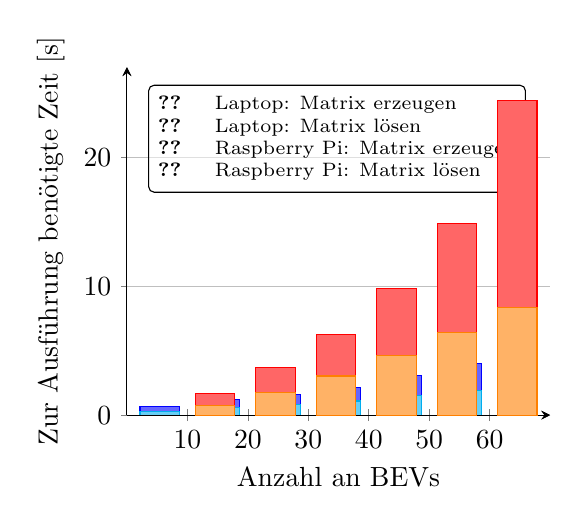
\begin{tikzpicture}
	\begin{axis}[
		ybar stacked,
		bar shift=-10pt,
		%nodes near coords,
		bar width=0.5cm,
		axis lines=left,
		height=6cm,
		xlabel={Anzahl an BEVs},
		ylabel={Zur Ausführung benötigte Zeit [s]},
		ymin=0,
		ymax=27,
		xmin=0,
		xmax=70,
		ymajorgrids,
		%symbolic x coords={a, b, c, d, e, f},
		xtick=data,
%		legend pos=north west,
%		legend style={
%			font=\scriptsize,
%			legend cell align=left
%		}
	]
		\addplot[fill=cyan!60, draw=cyan] coordinates{
			(10, 0.29) (20, 0.61) (30, 0.84) (40, 1.1) (50, 1.51) (60, 1.91)
		};
		\label{pgfplots:laptop-create-matrix}
		\addplot[fill=blue!60, draw=blue] coordinates{
			(10, 0.36) (20, 0.61) (30, 0.74) (40, 1.04) (50, 1.56) (60, 2.13)
		};
		\label{pgfplots:laptop-solve-matrix}
	\end{axis}
	
	\begin{axis}[
		ybar stacked,
		bar shift=10pt,
		%nodes near coords,
		bar width=0.5cm,
		axis lines=left,
		height=6cm,
		ymin=0,
		ymax=27,
		xmin=0,
		xmax=70,
		ymajorgrids,
		%symbolic x coords={a, b, c, d, e, f},
		ticks=none=data,
%		legend pos=north west,
%		legend style={
%			font=\scriptsize,
%			legend cell align=left
%		}
	]
		\addplot[fill=orange!60, draw=orange] coordinates{
			(10, 0.74) (20, 1.79) (30, 3.04) (40, 4.65) (50, 6.44) (60, 8.37)
		};
		\label{pgfplots:raspi-create-matrix}
		\addplot[fill=red!60, draw=red] coordinates{
			(10, 0.91) (20, 1.91) (30, 3.25) (40, 5.2) (50, 8.41) (60, 16.02)
		};
		\label{pgfplots:raspi-solve-matrix}
		
		\node[draw, fill=white, anchor=north west,
		rounded corners=2pt, fill opacity=0.5, draw opacity=1,
		text opacity=1] at (axis description cs: 
		0.05, 0.95){
			\scriptsize
			\begin{tabular}{@{}ll@{}}
				\ref{pgfplots:laptop-create-matrix} & Laptop:
				Matrix erzeugen\\
				\ref{pgfplots:laptop-solve-matrix} & Laptop:
				Matrix lösen\\
				\ref{pgfplots:raspi-create-matrix} & Raspberry Pi: Matrix
				erzeugen\\
				\ref{pgfplots:raspi-solve-matrix} & Raspberry Pi: Matrix
				lösen\\
			\end{tabular}
		};
	\end{axis}
\end{tikzpicture}